% Created 2013-12-20 金 04:52
\documentclass[12pt]{jsarticle}
\usepackage[dvipdfmx]{graphicx}
\usepackage{comment}
%\usepackage{setspace}
%%\date{\today}
%\title{}
\textheight = 25truecm
\textwidth = 18truecm
\topmargin = -1.5truecm
\oddsidemargin = -1truecm
\evensidemargin = -1truecm
\marginparwidth = -1truecm
\def\theenumii{\Alph{enumii}}
\def\theenumiii{\alph{enumiii}}
\def\labelenumi{(\theenumi)}
\def\labelenumiii{(\theenumiii)}
%\setstretch{0.9}
\begin{document}

%\maketitle
%\tableofcontents

\begin{center}
%%%%%%%%%%%%%%%%%%%%%%%%%%%%%%%%%%%%%%%
%%%タイトル                         %%%
%%%%%%%%%%%%%%%%%%%%%%%%%%%%%%%%%%%%%%%
{\LARGE NICドライバの改変(途中経過)}
\end{center}

\begin{flushright}
  2014/10/31\\
  藤田将輝
\end{flushright}
%%%%%%%%%%%%%%%%%%1章%%%%%%%%%%%%%%%%%%%
\section{はじめに}

NICドライバの割り込み処理を対象としたデバッグ支援環境の実装をするため,
実験を行っている.
本資料では本機構の実装における実験項目とその途中経過を示す.
なお,NICドライバはRTL8169を用いている.

\section{実験項目}
本機構における実装目標を図1に示す.
また,これを実現するための実験項目とその進捗状況,および目標との対応を表1にまとめた.
なお,図1については前回の資料で説明しているため,説明を省く.

\begin{table}[htb]
\caption{実験項目}
\begin{center}
  \begin{tabular}{c|p{8cm}|c|r} \hline
    項目 & 実験項目 & 進捗状況 & 図1との対応 \\ \hline \hline
    A & 割り込み情報を指定し,デバッグ支援機構に通知するプログラムを作成する & 未着手 & (1)(2) \\ \hline
    B & パケットを共有メモリの受信バッファに格納する & 途中 & (3)(4) \\ \hline
    C & IPIを受信すると動作し,NICドライバ内の関数を呼び出す割り込みハンドラを作成する & 未着手 & (6)(7)(8) \\ \hline
    D & 保存していたパケットの情報からNICの通信なしで受信処理を発生させ,割り込み処理を再現する & 途中 & (9)(10) \\ \hline
    E & Mintの共有メモリに受信ディスクリプタを作成する & 未着手 & (5)(9) \\ \hline
    F & NICデバイスドライバにおいて確認する受信ディスクリプタをMint上に作成した受信ディスクリプタにする & 未着手 & (9) \\ \hline
  \end{tabular}
  \end{center}
\end{table}



\begin{figure}[t]
\begin{center}
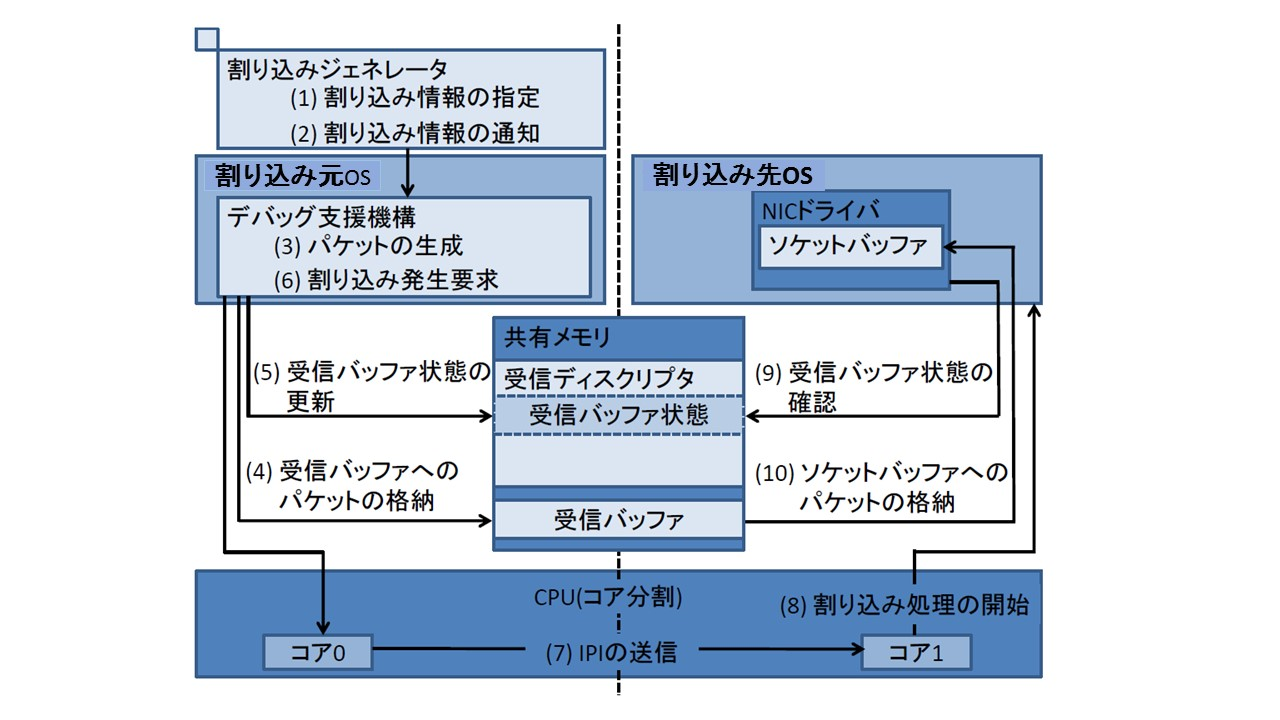
\includegraphics[height=8.0cm]{./fig1.jpg}          
\caption{実装目標}
\label{fig:up}
\end{center}
\end{figure}

以降の章からは表1の(B)(D)の途中経過を示す.



\section{(B)について}
\subsection{最終目標}
送信したいパケットをNICを使用せずにMintの共有メモリに格納する.
\subsection{実験の流れ}
NICドライバ内の送信処理の関数であるrtl8169\_start\_xmit()内でパケットをMintの共有メモリ内に格納し
確認する.
\subsection{途中経過}
NICドライバのパケット送信処理において,パケットの送信処理の関数であるrtl8169\_start\_xmit()内で
パケット内のデータを共有メモリに格納し,これを確認した.
なお,格納されるのは最後に送信されたパケットのみである.

\subsection{確認方法}
3.2節で述べたパケットを確認するため,指定したメモリ領域から文字列を取得し,取得した文字列をカーネルコンソールに
表示するシステムコールを作成し,使用した.
このシステムコールを使用し,dmesgを確認するとパケットの中身らしきものが表示されていた.
今後は表示されたものがパケットの中身として正しいのかどうかを確認する.
また,Mintの共有メモリ内で,リングバッファを実装し,NICドライバの受信バッファとする.

\section{(D)について}
\subsection{最終目標}
NICドライバの受信割り込み処理をNICなしで発生させる.
\subsection{実験の流れ}
送信側のマシンから受信側のマシンへパケットを送信する.
このパケットを保存,使用し,受信処理の再現をする.
\subsection{途中経過}
NICドライバ内で保存したパケットで
割り込み処理を再現する実験をしている.
具体的には,NICドライバが受信したパケットを複写し,保存しておき,
その保存したパケットを使用して,同じ処理を再現させるというものである.
現在は,送信側が送信したパケットだけでなく,他のマシンから送信されている多数のパケットも受信しているため,NICドライバレベルで
送信側が送信したパケットの特定ができていない.このため,パケットの特定方法を調査中である.

\section{おわりに}
本資料では,本機構実装における実験項目と,その進捗状況について示した.
以降は,実験項目を消化し,実装をすすめる.
\end{document}
